\documentclass{article}
\usepackage[a4paper, margin=1in]{geometry}
\usepackage[T1]{fontenc}
\usepackage[utf8]{inputenc}
\usepackage{amsmath, amssymb, graphicx, hyperref}
\graphicspath{{../figures/}}
\usepackage[framed,numbered]{matlab-prettifier}
\usepackage{xcolor}
\usepackage{bookmark}
\usepackage{listings}

\geometry{a4paper, margin=1in}

% MATLAB code style
\lstset{
  style      = Matlab-editor,
  basicstyle = \mlttfamily,
  breaklines = true
}

\title{\textbf{Practical - 11}}
\author{}
\date{October 29, 2026}

\pagenumbering{gobble}

\begin{document}
\maketitle

\noindent
\textbf{\large{Aim:}} To analyze a predator-prey model with density dependence.

\vspace{1em}
\noindent
\textbf{\large{Theory:}}

\vspace{0.5em}
\noindent
\textbf{Basic Concept}

\noindent
In the basic Lotka–Volterra model, prey can grow exponentially when predators are absent. This assumes unlimited resources. In reality, food, water and space are limited. Density dependence means that the growth rate of a population depends on its population size.

\noindent
As the prey population grows, competition for limited resources reduces its growth rate. This can be represented using logistic growth.

\vspace{1.5em}
\noindent
\textbf{Mathematical Model}

\noindent
Let $x(t)$ be the prey population and $y(t)$ be the predator population. We use the following commonly used model, where density dependence acts on the prey population:
\[\frac{dx}{dt} = ax(1 - \frac{x}{K}) - bxy\]
\[\frac{dy}{dt} = cxy - dy\]
Here, $a$ is the natural growth rate of prey, $K$ is the carrying capacity of the environment, $b$ is the rate of prey loss due to predator interactions, $c$ measures predator growth supported by prey, and $d$ is the natural death rate of predators.

\begin{table}[h]
    \centering
    \begin{tabular}{|c|c|}
    \hline
    \textbf{Symbol} & \textbf{Meaning} \\
    \hline
    \textbf{$x(t)$} & Prey population at time $t$ \\
    \hline
    \textbf{$y(t)$} & Predator population at time $t$ \\
    \hline
    \textbf{$a$} & Intrinsic growth rate of prey \\
    \hline
    \textbf{$K$} & Carrying capacity of the environment \\
    \hline
    \textbf{$b$} & Predation coefficient \\
    \hline
    \textbf{$c$} & Predator growth coefficient due to prey consumption \\
    \hline
    \textbf{$d$} & Natural death rate of predators \\
    \hline
    \end{tabular}
\end{table}

\vspace{1.5em}
\noindent
\textbf{Equations}

\noindent
Prey equation: $\frac{dx}{dt} = ax(1 - \frac{x}{K}) - bxy$.

\noindent
The term $ax(1 - \frac{x}{K})$ describes logistic prey growth. When $x$ is small compared with $K$, prey can grow quickly. As $x$ approaches $K$, natural growth slows. The term $-bxy$ represents prey loss due to predators.

\vspace{0.5em}
\noindent
Predator equation: $\frac{dy}{dt} = cxy - dy$.

\noindent
The term $cxy$ represents predator growth supported by feeding on prey, while $-dy$ represents natural predator deaths.

\vspace{1em}
\noindent
\textbf{\large{MATLAB Code:}}
\begin{lstlisting}
clc; clear all; close all;

a = 1.0;
K = 250;
b = 0.02;
c = 0.01;
d = 0.5;

x0 = 40;
y0 = 9;

tspan = [0,50];
initial = [x0, y0];

f = @(t,z)[a*z(1)*(1 - z(1)/K) - b*z(1)*z(2);
    c*z(1)*z(2) - d*z(2)];

[t,Z] = ode45(f, tspan, initial);

x = Z(:,1);
y = Z(:,2);

plot(t,x,'LineWidth',1.5)
hold on
plot(t,y,'LineWidth',1.5)
grid on
xlabel('Time')
ylabel('Population')
title('Predator-Prey Model with Density Dependance')
legend('Prey Population', 'Predator Population', 'Location','best')
hold off
\end{lstlisting}

\vspace{1em}
\noindent
\textbf{\large{Output:}}
\begin{figure}[htbp]
    \centering
    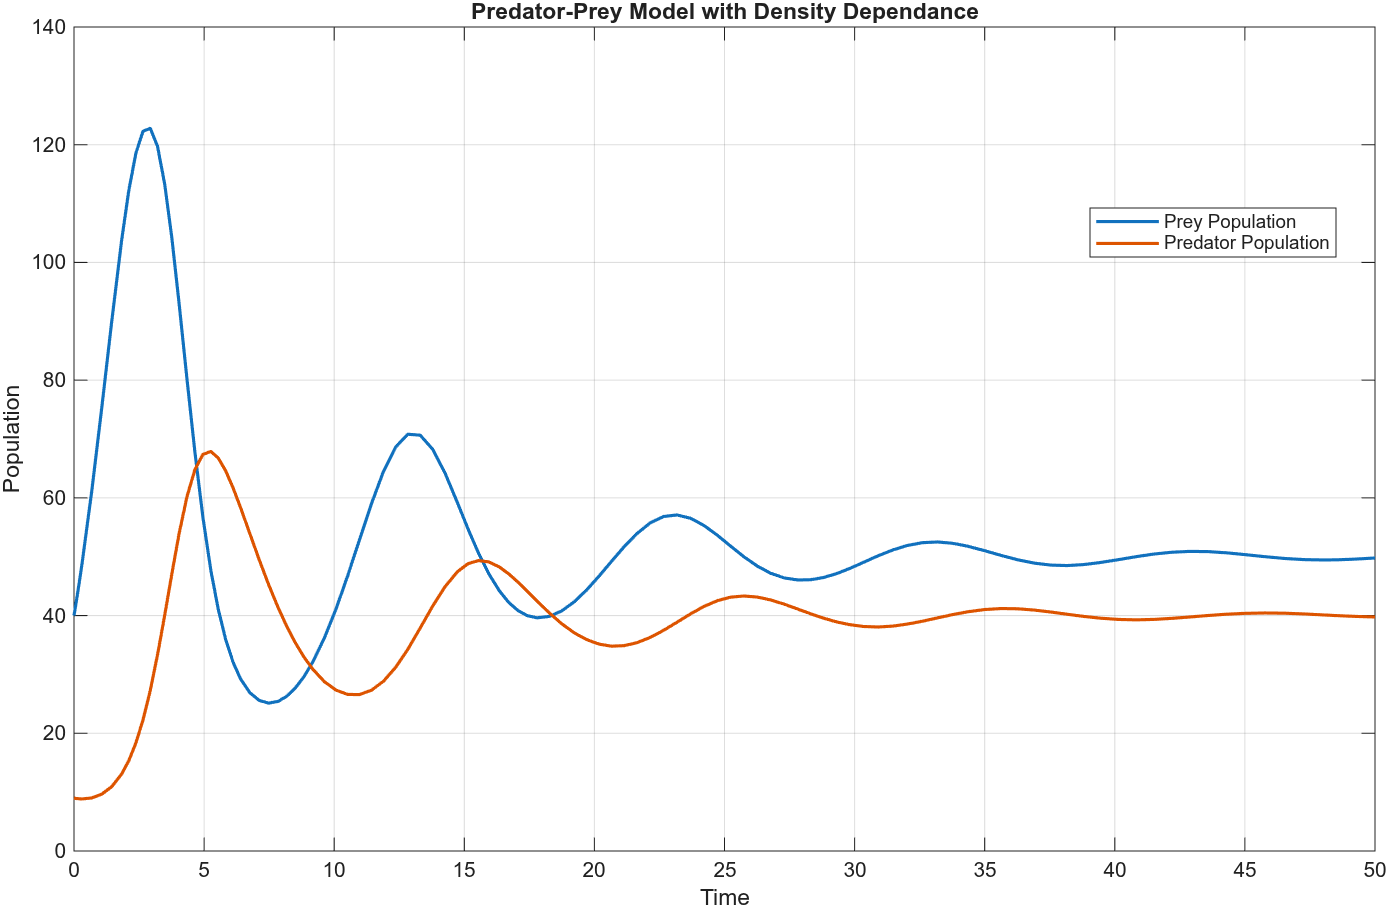
\includegraphics[width=0.7\textwidth]{Figure11.png}
\end{figure}

\vspace{1em}
\noindent
\textbf{Graph Interpretation:}

\noindent
The prey population is limited by the carrying capacity $K$, so it does not follow unrestricted exponential growth. Predator numbers depend on the availability of prey. Depending on the parameters, the populations may fluctuate, settle toward an equilibrium, or show other transient behaviour. The exact result depends on parameter values and initial populations.

\end{document}
